% ------------------------------------------------------------------------
% ------------------------------------------------------------------------
% ------------------------------------------------------------------------
\chapter{MCM 2025}


% ------------------------------------------------------------------------
\section{Welcome to MCM 2025}

We are delighted to welcome you to Chicago for the \emph{16th International Conference on Monte Carlo and Quasi-Monte Carlo Methods in Scientific Computing}. The MCM conference series is, together with its sister conference series, the conferences on Monte Carlo Methods (MCM), a major event for researchers in the Monte Carlo and quasi-Monte Carlo community. We are glad to host MCM in Canada for a second time, the first being held in Montr\'{e}al (2008).


MCM 2025 marks the thirty-year anniversary of the first MCM conference held in 1994. To celebrate this milestone, the organizing committee are excited to present a special panel session, followed by a Q\&A. The panel members consist of Art Owen, Fred Hickernell, Frances Kuo, Alexander Keller and Josef Dick and the session will be moderated by Aretha Teckentrup. The motivation and purpose of this special event is to reflect on the past thirty years of progress in the field of MC and QMC methods and perhaps more importantly, to look ahead to what the big questions might reveal in the next thirty years and beyond.

As of July 5th, MCM 2024 features 137 talks, 
among them eight plenary talks, two tutorials, and twenty-four special sessions. 
The speakers come from a variety of scientific backgrounds, countries, institutions and stages of their career. 

Located in South-West Ontario on the Grand River, Waterloo, or more widely known as part of the twin-cities of Kitchener-Waterloo (KW), offers cultural richness and technological innovation. Celebrated for its bustling tech scene, Waterloo has rightfully earned its part in the nickname "Silicon Valley North." In addition, KW boasts a rich cultural scene, highlighted by the annual Oktoberfest, the largest celebration of its kind outside of Germany. We hope that you enjoy what KW has to offer you away from campus!

We wish you a productive and interesting week at MCM 2024!


\bigskip
\emph{Fred Hickernell, Sou-Cheng Choi, Nathan Kirk, etc.} \\
MCM 2025 Conference Organizers \\

% \colorbox{gray!20!white}{\makebox{%
%   \includegraphics[width=3cm]{organizer-Sloan}\;%
%   \includegraphics[width=3cm]{organizer-Kuo}\;%
%   \includegraphics[width=3cm]{organizer-Dick}\;%
%   \includegraphics[width=3cm]{organizer-Peters}%
%   }}



\vspace{5cm}
Conference website: \url{https://ccbatiit.github.io/mcm2025/} \\
\\
Conference email: \url{info@mcm2025chicago.org}

% ------------------------------------------------------------------------
\thispagestyle{empty} \tableofcontents

\section{About MCM}

\subsection{History}

The MCM Conference is a biennial meeting devoted to the study of Monte
Carlo (MC) and quasi-Monte Carlo (QMC) methods, the relationships between
the two classes of methods, and their effective application in different
areas. Consistently attracting between one-hundred and two-hundred participants in recent years, its aim
is to provide a forum where leading researchers and users can exchange
information on the latest theoretical developments and important
applications of these methods. The conference focuses primarily
on the mathematical study of these techniques, their implementation and
adaptation for concrete applications, and their empirical assessment.

The conference was initiated by Harald Niederreiter, who co-chaired the
first seven conferences of the series. From 2006 onwards, the MCM Steering Committee has
overseen the continuation of the conference series.

The previous instances of MCM were held in:
\begin{enumerate}
\item Las Vegas, USA (1994),
\item Salzburg, Austria (1996),
\item Claremont, USA (1998),
\item Hong Kong (2000),
\item Singapore (2002),
\item Juan-Les-Pins, France (2004),
\item Ulm, Germany (2006),
\item Montr\'{e}al, Canada (2008),
\item Warsaw, Poland (2010),
\item Sydney, Australia (2012),
\item Leuven, Belgium (2014),
\item Stanford, USA (2016),
\item Rennes, France (2018),
\item Oxford, UK (2020, virtually),
\item Linz, Austria (2022).
\end{enumerate}

\iffalse
%% NK: moved to 'Welcome' on May 7
\vspace{0.25cm}
MCM 2024 marks the thirty-year anniversary of the first MCM conference held in 1994. To celebrate this milestone, the organizing committee of MCM 2024 are excited to present a special panel session, followed by a Q\&A. The panel members consist of Art Owen, Fred Hickernell, Frances Kuo, Alexander Keller and Josef Dick and the session will be moderated by Aretha Teckentrup. The motivation and purpose of this special event is to reflect on the past thirty years of progress in the field of MC and QMC methods and perhaps more importantly, to look ahead to what the big questions might reveal in the next 30 years and beyond.
\fi

\newpage
\subsection{Steering Committee}

\setlength{\columnsep}{1cm}
\begin{multicols}{2}
%\small
\raggedright

Josef Dick (Australia)

Fred J. Hickernell (USA)

Alexander Keller (Germany, Chair)

Peter Kritzer (Austria)

Pierre L'Ecuyer (Canada)

Christiane Lemieux (Canada)

Art B. Owen (USA)


\end{multicols}

\clearpage

\subsection{Scientific committee}



\setlength{\columnsep}{1cm}
\begin{multicols}{2}
\raggedright
Christoph Aistleitner (Graz University of Technology, Austria)

Andrea Barth (University of Stuttgart, Germany)

Hector Cancela (University of the Republic, Uruguay)

Frédéric Cérou (INRIA, France)

Nicolas Chopin (ENSAE, IPP, France)

Ronald Cools (KU Leuven, Belgium)

Josef Dick (UNSW, Australia)

Mike Giles (Mathematical Institute, University of Oxford, UK)

Paul Glasserman (Columbia University, USA)

Michael Gnewuch (University of Osnabrück, Germany)

Takashi Goda (University of Tokyo, Japan)

Stefan Heinrich (RPTU Kaiserslautern-Landau, Germany)

Fred J. Hickernell (Illinois Institute of Technology, USA)

Alexander Keller (NVIDIA, Germany)

Peter Kritzer (RICAM, Austrian Academy of Sciences, Austria)

Dirk Kroese (University of Queensland, Australia)

Frances Kuo (UNSW, Australia)

Gerhard Larcher (JKU Linz, Austria)

Christian Lécot (Université Savoie Mont-Blanc, France)

Pierre L'Ecuyer (University of Montreal, Canada)

Faming Liang (Purdue University, USA)

Eric Moulines (\'{E}cole Polytechnique, France)

Thomas Müller-Gronbach (University of Passau, Germany)

Harald Niederreiter (RICAM, Austrian Academy of Sciences, Austria)

Erich Novak (FSU Jena, Germany)

Art Owen (Stanford University, USA)

Gilles Pagès (Sorbonne Universit\'{e}, France)

Friedrich Pillichshammer (JKU Linz, Austria)

Michael Pitt (King's College London, UK)

Sebastian Reich (University of Potsdam, Germany)

Klaus Ritter (Fachbereich Mathematik, TU Kaiserslautern, Germany)

Gerardo Rubino (INRIA, France)

Claudia Schillings (Free University Berlin, Germany)

Wolfgang Schmid (Paris Lodron University of Salzburg, Austria)

Ian H. Sloan (UNSW, Australia)

Aretha Teckentrup (University of Edinburgh, UK)

Bruno Tuffin (INRIA, France)

Mario Ullrich (JKU Linz, Austria)

Arne Winterhof (RICAM, Austrian Academy of Sciences, Austria)

\end{multicols}




\clearpage



\subsection{Local Organizers}
\update{}

Christiane Lemieux, Ben Feng, Nathan Kirk, Adam Kolkiewicz

\subsection{Local Technical and Support Team}
Greg Preston, Carla Daniels, Carlos Mendes, Lucy Simpson

% \colorbox{gray!20!white}{\makebox{%
%   \includegraphics[width=3cm]{organizer-Sedgers}}}

\subsection{Sponsors}



Fields Institute for Research in Mathematical Sciences\\
\url{http://www.fields.utoronto.ca}

Royal Bank of Canada (RBC)\\
\url{https://www.rbcroyalbank.com}

Faculty of Mathematics, University of Waterloo\\
\url{https://uwaterloo.ca/math}

Department of Statistics and Actuarial Science, University of Waterloo\\
\url{https://uwaterloo.ca/statistics-and-actuarial-science}\\

\begin{figure}[ht]
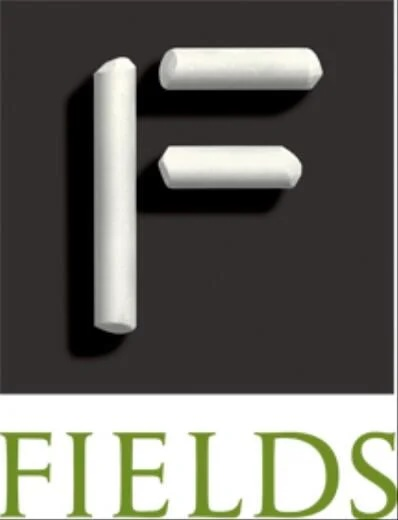
\includegraphics[scale =0.2]{Photos/fields_logo_extralarge}
\hfill

\includegraphics[scale =0.5]{Photos/UW.png}
\hfill
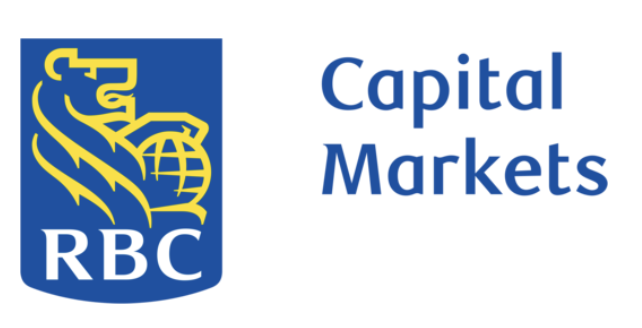
\includegraphics[scale =0.5]{Photos/RBC.png}
\end{figure}

\bigskip
\bigskip
\bigskip
% \begin{center}
% \includegraphics[height=3cm]{logomaths}\quad
% \includegraphics[height=3cm]{logoaustms}\quad
% \includegraphics[height=3cm]{logoanziam}
% 
% \bigskip
% \includegraphics[height=3cm]{logoamsi}\quad
% \includegraphics[height=3cm]{logocsiro}\quad
% \includegraphics[height=3cm]{logonsf}
% \end{center}

\clearpage
% ------------------------------------------------------------------------
\subsection{Special Thanks}

The conference organizers would like to thank all sponsors for making this
event possible. We also want to express our gratitude towards 
Professors Stefan Steiner and Changbao Wu (former and current Department Chair of Statistics and Actuarial Science at the University of Waterloo) and Professor Mark Giesbrecht (Dean, Faculty of Mathematics) for providing us with resources to help with the organization of this conference. We also thank the University of Waterloo for providing us with the space needed to host this conference.


We are also very grateful to our staff colleagues in the Department of Statistics and Actuarial Science for their unwavering assistance with many aspects of the organization, with special thanks in particular to Greg Preston, as well as Carla Daniels, Anthea Dunne, Carlos Mendes and Lucy Simpson.


We wish to extend our thanks to the entire Steering Committee and
Scientific Program Committee, and past MCM conference organizers for their
contribution and support. We also thank our plenary speakers, tutorial
speakers, special session organizers, and all session chairs for their
help and support with the scientific organisation of the conference. We are particularly grateful to Alex Keller, Frances Kuo, Peter Kritzer and  Art Owen for providing detailed feedback and suggestions based on their past experience with the organization of the MCM conference.

\clearpage

%Last but not least, we are extremely grateful to many friends in the MCM community 
%who helped us in various ways to organize MCM 2022, in particular Mike Giles, 
%Takashi Goda, Fred J. Hickernell, Frances Y. Kuo, Christiane Lemieux, and Art B. Owen. 

% ------------------------------------------------------------------------
% ------------------------------------------------------------------------
% ------------------------------------------------------------------------